\documentclass[addpoints ]{exam}

\usepackage{amssymb, amsmath, amsfonts}
\usepackage{geometry}
\usepackage{graphicx}
\usepackage{tikz}
\usetikzlibrary{calc}
\usepackage{multirow,array} % for payoff matrix formatting

\definecolor{crimson}{RGB}{ 170, 4, 36 }
\definecolor{darkblue}{RGB}{ 4, 47, 170 }
\definecolor{brown}{RGB}{ 111, 71, 2 }
\definecolor{periwinkle}{RGB}{ 90, 177, 204 }
\definecolor{ducksgreen}{HTML}{007030}

\geometry{left=1.0in,right=1.0in,top=1.0in,bottom=1.0in}
\pagestyle{headandfoot}
\lhead{EC327 Game Theory}
\chead{Homework 2}
\rhead{Winter 2024}
\runningheadrule

\title{
    \textbf{Econ 327: Game Theory} \\ 
    Homework $\#2$
    }
\author{University of Oregon}
\date{Due: Feb. 6$^{th}$}

% exam-type question formatting
\renewcommand{\thequestion}{\textbf{Question \arabic{question}}}
\bracketedpoints

\begin{document}

\maketitle

\begin{center}
  \gradetable[h][questions]
\end{center}

\vspace{0.5in}

\begin{center}
  \textbf{For homework assignments:}
\end{center}

\begin{itemize}

%  \item DO NOT write your name:
%  this assignment will be graded anonymously. 
%  If you want to, you can include your student ID instead.

  \item Complete \textit{all} questions and parts.
  I will select one question at random to be graded
  according to the rubric on Canvas.

  \item You may choose to work with others,
  but everyone must submit to Canvas individually.
  Please include the names of everyone who you worked with 
  below your own name.
 
\end{itemize}

\vspace{1.0in}

\makebox[.6\textwidth]{Name\enspace\hrulefill}

\vspace{0.5in}

% \begin{center}
%   \fbox{\fbox{\parbox{5.5in}{\centering
%     Answer the questions in the spaces provided on the
%     question sheets. If you run out of room for an answer,
%     continue on the back of the page or another sheet of paper.}}}
% \end{center}

\newpage

\begin{questions}

%------------------------------------------------------------------%

\question[10]
\textbf{Multiple Choice}

\begin{parts}

  \part Consider the strategic form game below:
  \begin{table}[h!]
    \begin{center}
    \begin{tabular}{*{4}{c|}}
      \multicolumn{2}{c}{} & \multicolumn{1}{c}{$Oregon~Driver$} \\\cline{3-4}
      \multicolumn{1}{c}{} & & $Swerve$ & $Straight$ \\\cline{2-4}
      \multirow{2}*{$California~Driver$}  & $Swerve$ & -1,-1 & 1,1 \\\cline{2-4}
                           & $Straight$ & 1,1 & -1,-1 \\\cline{2-4}
    \end{tabular}
    \end{center}
  \end{table}

  What type of game is this?
  \begin{choices}
    \choice A zero-sum game
    \choice A coordination game 
    \CorrectChoice An anti-coordination game
    \choice A prisoners' dilemma
  \end{choices}

  \part Consider the strategic form game below:
  \begin{table}[!h]
  \begin{center}
    \begin{tabular}{*{4}{c|}}
      \multicolumn{2}{c}{} &
      \multicolumn{1}{c}{Navratilova} \\ \cline{3-4}
      \multicolumn{1}{c}{} & & $DL$ & $CC$ \\ \cline{2-4}
      \multirow{2}*{Evert} & $DL$ & 50, 50 & 80, 20 \\ \cline{2-4}
        & $CC$ & 90,10 & 20, 80 \\ \cline{2-4} 
    \end{tabular}
  \end{center}
  \end{table}

  Which method would you use to solve for Nash equilibria?
  \begin{choices}
    \CorrectChoice Graphing mixed strategies
    \choice Iterative deletion of strictly dominated strategies 
    \choice Backwards induction
    \choice There are no Nash equilibria of this game.
  \end{choices}

  \part Cosider the same game as above.
  Suppose that Navratilova plays $DL$ with probability $p$ 
  and $CC$ with probability $(1-p)$.
  What are Evert's expected payoffs?

  \begin{choices}
    \choice $U_{Evret}(DL) = 30 - 80p$, $U_{Evret}(CC) = 70 - 20p$
    \CorrectChoice $U_{Evret}(DL) = 80 - 30p$, $U_{Evret}(CC) = 20 + 70p$
    \choice $U_{Evret}(DL) = - 60p$, $U_{Evret}(CC) = 100 + 100p$
    \choice $U_{Evret}(DL) = 90 - 40p$, $U_{Evret}(CC) = 20 + 60p$
  \end{choices}


  \part The difference between a regular Nash equilibrium 
  and a Subgame Perfect Nash equilibrium is that:

  \begin{choices}
    \choice A Subgame Perfect Nash equilibrium assumes perfect information
    \choice Mixed strategies cannot be used in Subgame Perfect Nash equilibria
    \CorrectChoice Subgame Perfect Nash equilibria assume that players won't fall for non-credible threats
    \choice There is no difference, they are the same
  \end{choices}

  \part Which of the following are examples of \textit{continuous} strategies?
  
  \begin{choices}
    \choice Taylor Swift's choice of which cities to go on tour in
    \CorrectChoice How much time Owen waits in line for Taylor Swift tickets
    \CorrectChoice How much money TicketMaster charges for a ticket
    \choice Jose is at home and will only go if the stadium is less than 50\% full
    \CorrectChoice Both B and C are continuous strategies
    \choice None of the above are continous strategies
  \end{choices}
\end{parts}
  
\newpage

%------------------------------------------------------------------%

\question
Consider the extensive form game treee below.

\begin{center}
  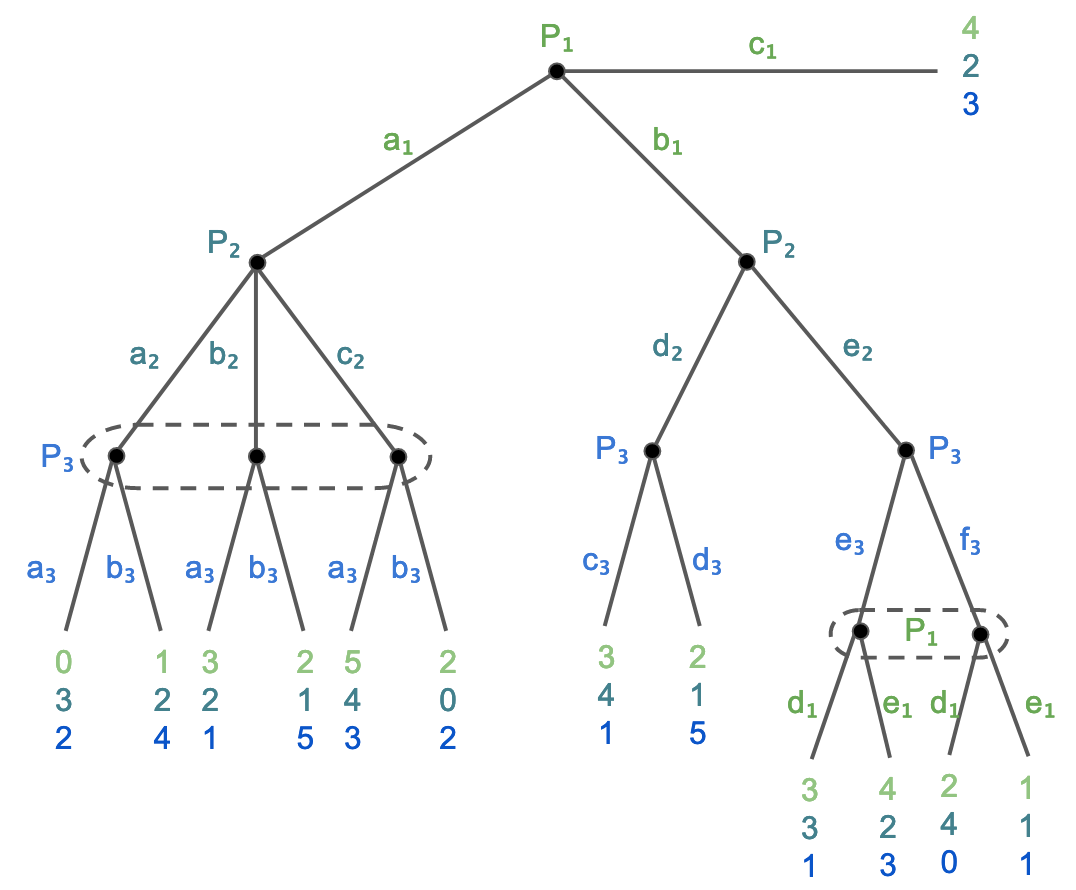
\includegraphics[width = .8\textwidth]{figures/gametree1.png}
\end{center}

\begin{parts}
  
  \part[1] 
  What should a complete strategy profile look like?

  How many elements will each player have in their \textit{complete} strategy?

  \part[6] Find all subgame perfect Nash equilibria in pure strategies.

  \part[3] Can you find a Nash equilibrium that is not subgame perfect?
  Carefully explain.

\end{parts}

\newpage

%------------------------------------------------------------------%

\question[10] 
A game theorist is walking down the street in his neighborhood and finds \$20.
Just as he picks it up, two neighborhood kids, 
Jane and Tim,
run up to him, asking if they can have it.
Because game theorists are generous by nature, 
he says he's willing to let them have the \$20,
but only according to the following procedure:
Jane and Tim are each to submit a written request 
as to their share of the \$20. 
Let $t$ denote the amount that Tim requests for himself
and $j$ be the amount that Jane requests for herself.
Tim and Jane must choose $j$ and $t$ from the interval
$[0,20]$.
If $j + t \leq 20$, then the two receive what they requested,
and the remainder, $20 - j - t$, is split equally between them.
If, however, $j + t > 20$, then they get nothing, and the game theorist keeps the \$20.
Tim and Jane are the players in this game.
Assume that each of them has a payoff equal to the amount of money that he or she receives. 
Find all Nash equilibria.
\footnote{Harrington \textit{Games, Strategies, and Decision Making}}

%\vspace{-5cm}

\newpage

%------------------------------------------------------------------

\question 

Consider a situation in which a student can decide to cheat or be honest on an exam.
If the faculty thinks the student has cheated, 
the faculty member has to decide whether to expel them from the college
or refer them to the Honor Board. 
The Honor Board has to decide whether to expel the student or find them innocent.
The payoffs are ordered, student, faculty, and college.
Assume the board shares the college's payoffs. 
\footnote{Cliff Bekar, Lewis and Clark College}

\begin{figure}[!h]
  \centering
  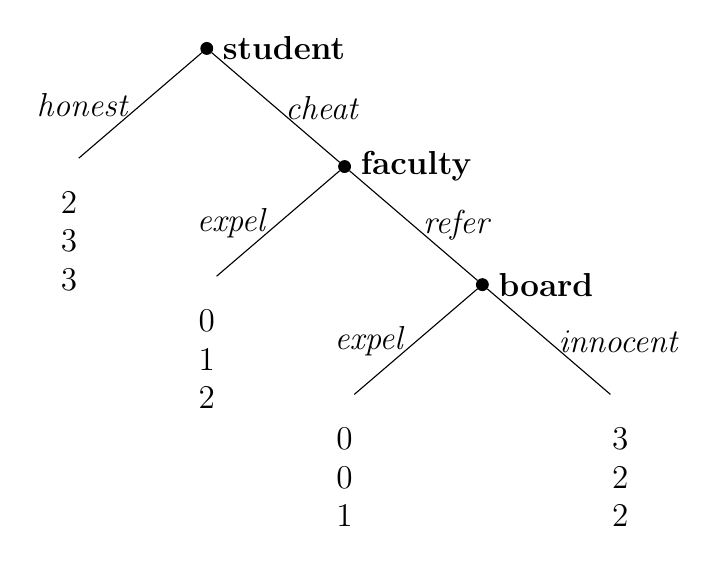
\begin{tikzpicture}[scale=1.0,font=\large]
\tikzstyle{solid node}=[circle,draw,inner sep=1.5,fill=black]
\tikzstyle{level 1}=[level distance=15mm,sibling distance=3.5cm]
\tikzstyle{level 2}=[level distance=15mm,sibling distance=3.5cm]
\tikzstyle{level 3}=[level distance=15mm,sibling distance=3.5cm]

\node(0)[solid node,label=right:{\textbf{student}}]{}
    child{node[label=below:{
            \begin{tabular}{c}
                 {2} \\
                 {3} \\
                 {3} \\
            \end{tabular}
        }]{} 
    edge from parent node[left]{\textit{honest}}}
    child{node[solid node,label=right:{\textbf{faculty}}]{} 
        child{node(1)[label=below:{
            \begin{tabular}{c}
                 {0}  \\
                 {1} \\
                 {2} \\
            \end{tabular}
        }]{} 
        edge from parent node[left]{\textit{expel}} 
        }
        child{node(2)[solid node, label=right:{\textbf{board}}]{} 
            child{node[label=below:{
                \begin{tabular}{c}
                    {0} \\
                    {0} \\
                    {1} \\
                \end{tabular}
                }]{} 
            edge from parent node[left]{\textit{expel}} 
            }
            child{node[label=below:{
                \begin{tabular}{c}
                     {3} \\
                     {2} \\
                     {2} \\
                \end{tabular}
            }]{} 
            edge from parent node[right]{\textit{innocent}} 
            }
        edge from parent node[right]{\textit{refer}} 
        }
    edge from parent node[right]{\textit{cheat}}
    };
    
\end{tikzpicture}

\end{figure}

\begin{parts}
  \part[2] Find the Subgame Perfect Nash Equilibrium.

  \part[6] Assume now that the board acts like $Nature$, making no deliberate choice 
  but instead expels a guilty student $q\%$ of the time.
  Find All SGPN as a function of $q$.

  \part[2] Relative to the pure threat of explusion alone, who gains and who loses
  from the existence of an honor board that expels probabalistically?

\end{parts}

\newpage

%------------------------------------------------------------------

\question

The players in the following game are $Bush$ and $Saddam$. 
$Bush$ suspects $Saddam$ of having Weapons of Mass Destruction (WMD).
Assume for the game that $Saddam$ does have WMD. 
$Bush$ can rely on $inspections$ or $invade$.
$Saddam$ can $hide$ his WMD or $destroy$ them.
\footnote{Cliff Bekar, Lewis and Clark College}

\begin{table}[h!]
  \begin{center}
  \begin{tabular}{*{4}{c|}}
    \multicolumn{2}{c}{} & \multicolumn{1}{c}{$Bush$} \\\cline{3-4}
    \multicolumn{1}{c}{} & & $Invade$ & $Inspect$ \\\cline{2-4}
    \multirow{2}*{$Saddam$}  & $Hide$ & -2,2 & 3,0 \\\cline{2-4}
                         & $Destroy$ & -1,-3 & 0,1 \\\cline{2-4}
  \end{tabular}
  \end{center}
\end{table}

\begin{parts}

  \part[4] 
  Plot the expected values of each player's relevant strategies and find the mixed strategy Nash probabilities.

  \part[4]
  Plot each agent's Best Response Functions. 
  Carefully:
  
  \begin{subparts}
    \subpart label your graph,
    \subpart indicate all Nash equilibria, 
    \subpart and explain your answer
  \end{subparts}

  \part[2]
  What is the probability Bush will invade only to find no WMD?
\end{parts}

%------------------------------------------------------------------

\end{questions}

\end{document}
